\chapter{Effets de taille finie}
    \label{chap-sos}

Certains dépôts de films nanoscopiques sur des surfaces présentent des fluctuations dont la longueur de corrélation est similaire à celle de la hauteur du film. L'interface entre le dépôt et le substrat présente une énergie libre qui dépend fortement de la taille dudit film\cite{ouyang_size-dependent_2006,jiang_size_2008}. De telles modifications des propriétés thermodynamiques à cause d'un effet de taille finie peut provoquer de fortes instabilités hydrodynamiques pouvant rendre le système thermodynamiquement instable\cite{ding_theoretical_2001}. Ces conditions aux limites entraînent une frustration du système qui finit par causer une force entre les surfaces du système, appelé force Casimir. Cette force entropique peut se retrouver dans les systèmes critiques\cite{} et possède alors des propriétés universelles selon la classe d'universalité du système. Plus proche des dépôts de film on retrouve les systèmes de membranes\cite{nelson_statistical_2004} possédant une force non-universelle\cite{hasnaoui_casimir_2010}. Certaines membranes biologiques possèdent même une transition de phase appartenant à la classe d'universalité du modèle d'Ising \cite{machta_critical_2012}.

Dès lors, quelles propriétés de la force de Casimir peut-on retrouver dans un modèle Solid-On-Solid d'Hamiltonien
\begin{align}
    \mH = J \sum_i |h_i-h_{i+1}| + \mu \frac{h_i+h_{i+1}}{2}
\end{align}
et avec quels outils peut-on l'étudier ?

%%%%%%%%%%%%%%%%%%%%%%%%%%%%%%%
\section{Limite thermodynamique}
%%%%%%%%%%%%%%%%%%%%%%%%%%%%%%




%%%%%%%%%%%%%%%%%%%%%%%%%

La fonction de partition d'un système dépend de la taille du système 
	
\begin{align}
    f_c(\beta,L,h) = - \frac{1}{L'} \frac{\delta \Omega(\beta,L,h)}{\delta L} \bigg|_{\beta,L'}
    \label{casimir-interface}
\end{align}	

parler problème localisation interface

Dans l'ensemble grand-canonique, la fonction de partition est calculée par les valeurs propres de la matrice de transfert de taille $L$ où l'on pose $\lambda_0 \ge \lambda_1 \ge ... \ge \lambda_n \ge 0$ :
\begin{align}
  \mZ =  \sum_\lambda \lambda^L 
\end{align}
Dans la limite thermodynamique $L \to \infty$, la fonction de partition se simplifie en $\mZ \simeq \lambda_0^L$.

\begin{figure}
	\begin{minipage}[t]{0.5\linewidth}
		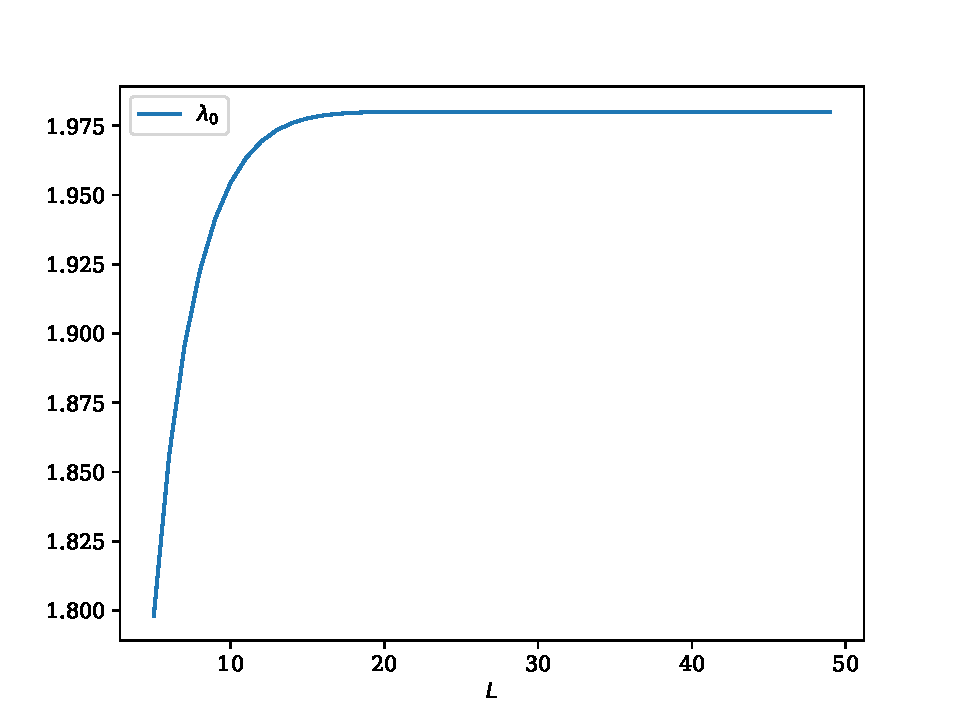
\includegraphics[width=\linewidth]{chap4/freeene-lambda0-mu.pdf}
	\end{minipage}%Cyclin
	\begin{minipage}[t]{0.5\linewidth}
		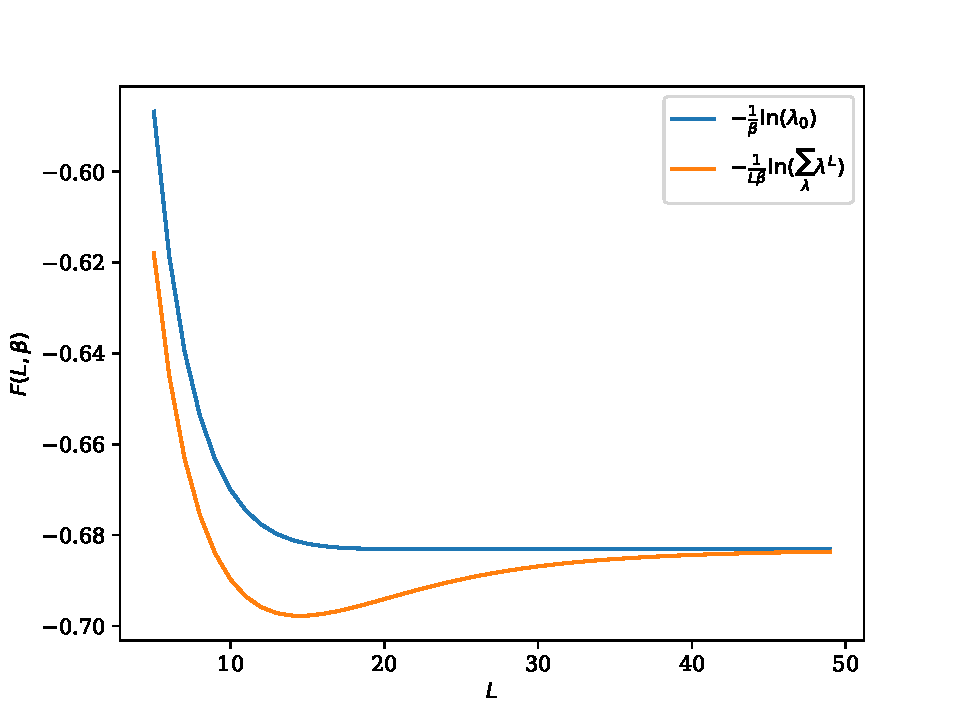
\includegraphics[width=\linewidth]{chap4/freeene-thermo-mu.pdf}
	\end{minipage}
	\centering
	\begin{minipage}{0.5\linewidth}
    	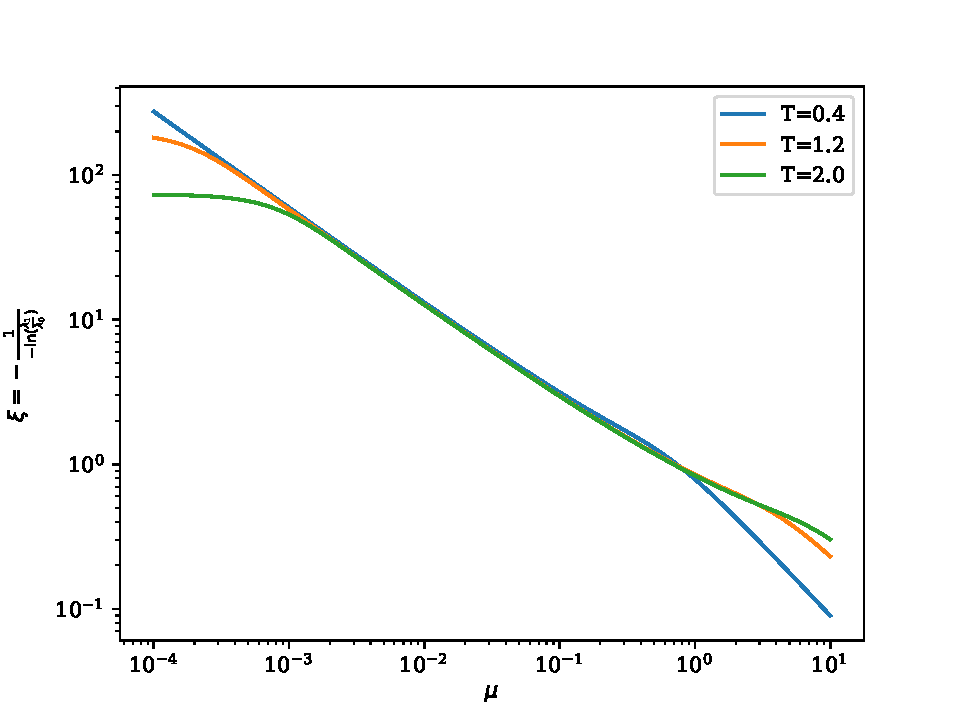
\includegraphics[width=\linewidth]{chap4/longueur-correl.pdf}
	\end{minipage}
	\caption{Plus grande valeur propre d'une interface libre en fonction de la taille $L$ du système pour $\mu = 0.01$ et $\beta = 1$ (gauche)  ; énergie libre par site calculée via l'approximation de la limite thermodynamique \ref{energie-libre-site} comparé à la vraie fonction de partition \ref{partition-trace-lambda} en fonction de la taille $L$ du système pour $\mu=0.01$ et $\beta = 1$ (droite) ; longueur de corrélation à grande distance \ref{longueur-correl-thermo} pour une matrice $200\times200$ en fonction du potentiel chimique $\mu$ pour différentes températures (bas).}
	\vspace{-0.5cm}
\end{figure}  
	
\begin{figure}
    \centering
	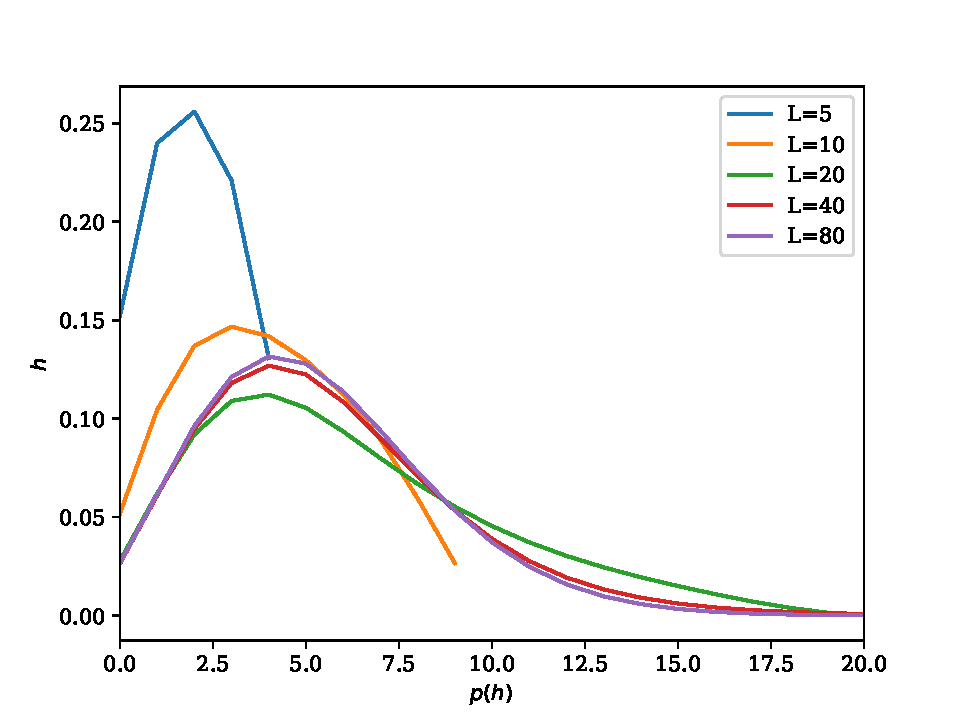
\includegraphics[width=0.5\linewidth]{chap4/distribution-taille-finie.pdf}
	\label{distribution-taille-finie}
	\caption{Distribution de l'interface pour différentes tailles de la matrice de transfert à $\mu=0.01$ et $\beta = 1$. Par un fit, la distribution ne suit pas une distribution de Poisson.}
\end{figure}

%%%%%%%%%%%%%%%%%%%%%%%%%%%%%%%%%%
\section{Effet Casimir}
%%%%%%%%%%%%%%%%%%%%%%%%%%%%%%%%%%

\begin{figure}
	\begin{minipage}[t]{0.5\linewidth}
		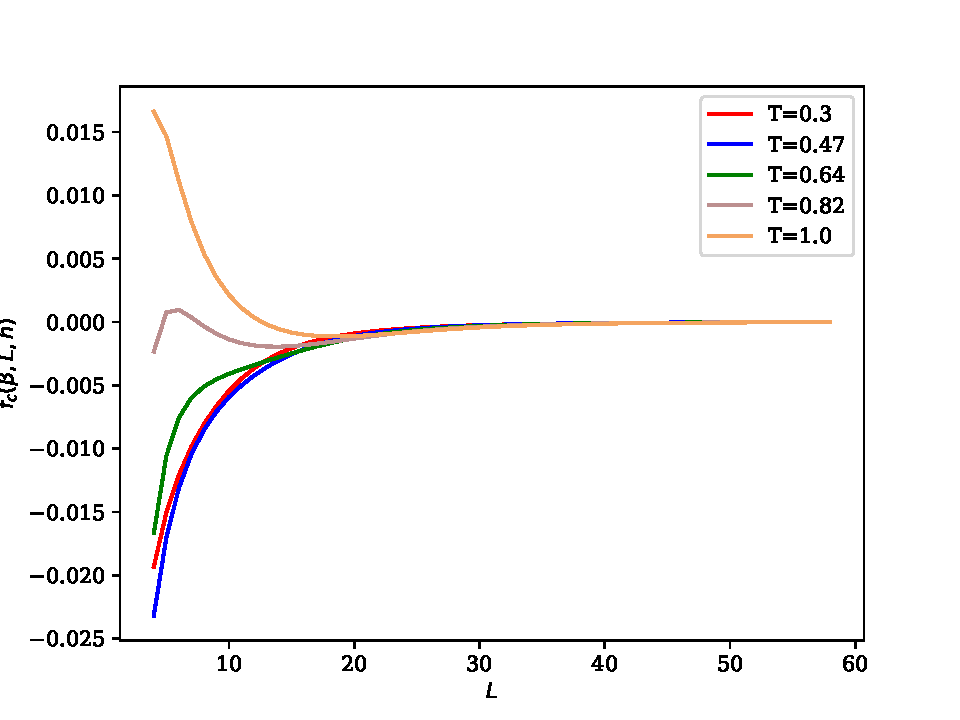
\includegraphics[width=\linewidth]{chap4/casimir-temperature-zoom.pdf}
	\end{minipage}%Cyclin
	\begin{minipage}[t]{0.5\linewidth}
		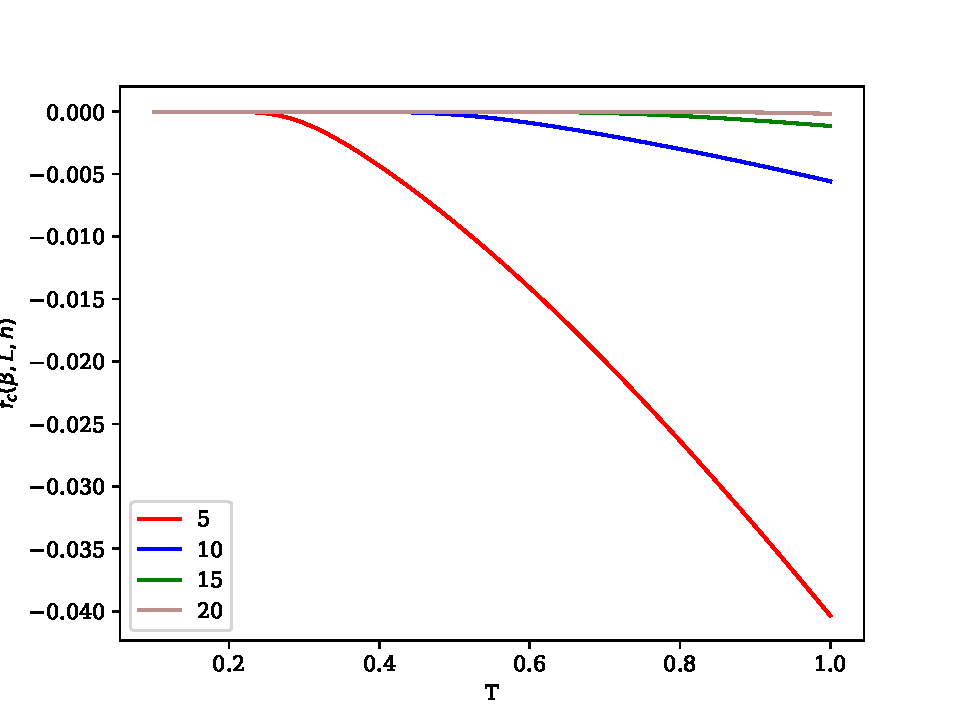
\includegraphics[width=\linewidth]{chap4/casimir-distance.pdf}
	\end{minipage}
	\centering
	\begin{minipage}{0.5\linewidth}
    	\includegraphics[width=\linewidth]{example-image-a}
	\end{minipage}	
	\label{casimir-temperature}
	\caption{Force de Casimir \ref{casimir-interface} en fonction de la distance pour $\mu = 0.01$ à température fixée (gauche) ; force de Casimir en fonction de la température pour $\mu=0.01$ à taille fixée (droite) ; force de Casimir en fonction du potentiel chimique pour $L=10$ à température fixée (bas). }
\end{figure}
    
%%%%%%%%%%%%%%%%%%%%%%%%%%%%%%%%%%
\section{Hamiltonien de transition}
\label{sec-transition}
%%%%%%%%%%%%%%%%%%%%%%%%%%%%%%%%%%

La force de Casimir dépend  de l'énergie libre, bien qu'elle ne puisse être exprimée par des moyennes d'observables facilement calculables par Monte Carlo. Néanmoins, sa dérivée peut être calculée via la méthode du paramètre de couplage. En suivant \cite{vasilyev_monte_2007,cardozo_finite_2015} pour un système d'Ising carré de taille $L \times L'$, l'idée est de calculer la dérivée continue par rapport à une taille discrète du système $L$ en interpolant le système via l'Hamiltonien de transition
\begin{align}
    \mH_{tr}(\lambda) = (1-\lambda) \mH_0 + \lambda \mH_1
    \label{hamil-trans}
\end{align}
où $\mH_0$ est l'Hamiltonien d'un système de hauteur maximale $L$, et $\mH_1$ l'Hamiltonien d'un système de hauteur maximale $L-1$ où on a découplé une couche (voir Figure \ref{decouplage}). L'énergie libre associée à cet Hamiltonien est
\begin{align}
    \Omega_{tr}(\lambda) = -k_B T \ln \left( \sum_{h_1 ... h_L} e^{-\beta \mH_{tr}(\lambda)} \right)
\end{align}
De la dérivée de l'énerie libre découle
\begin{align}
    \frac{\Omega_{tr}(\lambda)}{d\lambda} = < \mH_1 - \mH_0>_{\mH_{tr}(\lambda)}
\end{align}
où $< · >_{\mH_{tr}(\lambda)}$ représente la moyenne statistique sur le système en transition, facilement calculable dans les simulations numériques. En intégrant sur le couplage, on trouve au final que
\begin{align}
    \Omega_1 - \Omega_0 = \int_0^1 d\lambda  < \mH_1 - \mH_0>_{\mH_{tr}(\lambda)}
\end{align}
Finalement, dans la limite où l'épaisseur du système est suffisement grande pour que la variation d'une couche soit suffisement petite ($L' \gg 1$), on trouve que
\begin{align}
   - \frac{\partial \Omega(\beta,L,h)}{\partial L} \bigg|_{\beta,L'} \simeq  \int_0^1 d\lambda  < \mH_1 - \mH_0>_{\mH_{tr}(\lambda)}
\end{align}

\begin{figure}
	\begin{minipage}[t]{0.3\linewidth}
		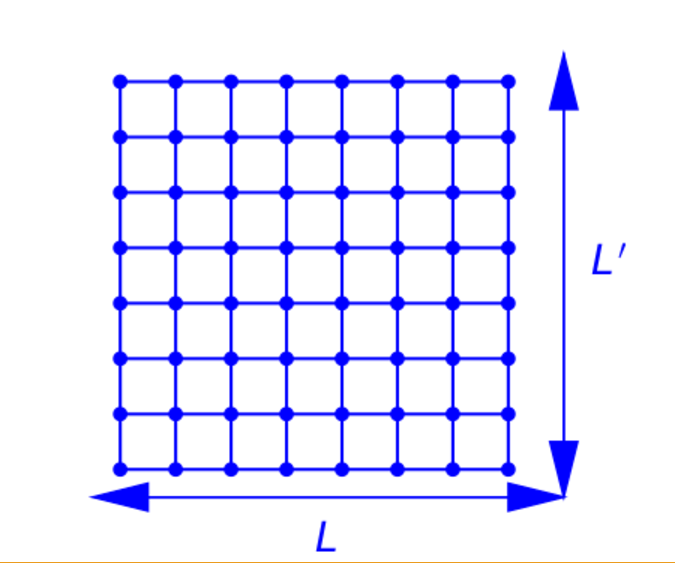
\includegraphics[width=\linewidth]{numerical/cross-h0.pdf}
		\caption*{$\mH_0$}
	\end{minipage}
	\begin{minipage}[t]{0.3\linewidth}
		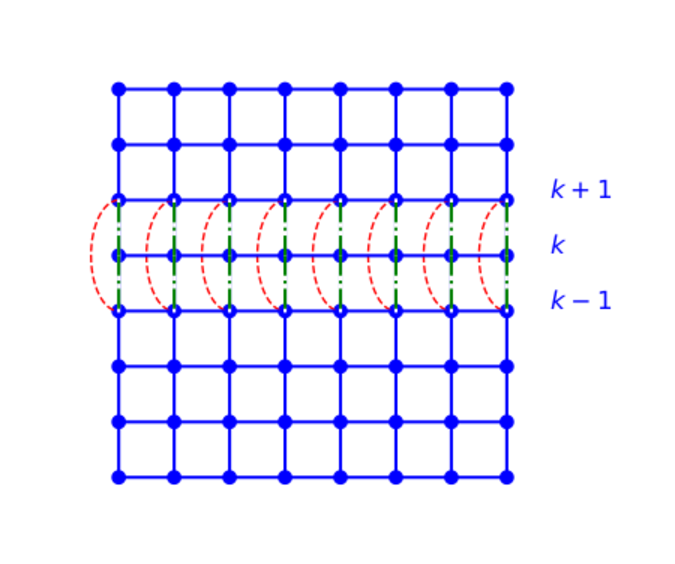
\includegraphics[width=\linewidth]{numerical/cross-hlambda.pdf}
		\caption*{$\mH(\lambda)$}		
	\end{minipage}
	\centering
	\begin{minipage}[t]{0.3\linewidth}
		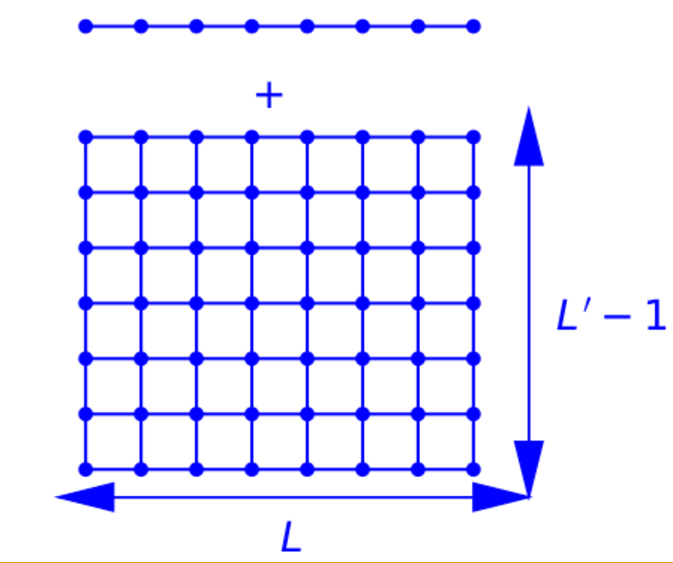
\includegraphics[width=\linewidth]{numerical/cross-h1.pdf}
		\caption*{$\mH_1$}
	\end{minipage}
	\caption{Découplage progressif de la $k$-ième couche du système afin de calculer la variation de l'énergie libre grâce à l'hamiltonien de transition. Les liens en bleu ont une énergie de $\beta J$, les liens en rouge une énergie de $\lambda \beta J $ et les liens en vert une énergie de $ (1-\lambda) \beta J$. Reproduction 2D de \cite{vasilyev_monte_2007}.}
	\label{decouplage}
\end{figure}

Pour le modèle Solid-On-Solid, il est possible de calculer la variation d'énergie créée par le découplage directement. Si le découplage s'est créé à la rangée $k$, on ajoute un lien d'énergie $\lambda J$ entre les rangées $k-1$ et $k+1$ et on retire $\lambda J$ énergie des rangées $k-1$ à $k$  et de $k$ à $k+1$. On obtient
\begin{align}
    &\mH_{tr,SOS}(\lambda) = \mH_{0,SOS} - \nn
     &\frac{\lambda J}{2} \sum_x \left[ \sgn(k-1-h(x)) \sgn(k+1-h(x)) - \sgn(k-h(x)) \left( \sgn(k-1-h(x))+\sgn(k+1-h(x)) \right) \right]
\end{align}
où le facteur $\frac{1}{2}$ est obtenu afin de prendre en compte le coefficient $2$ dans \ref{energie-sos-ising}. En faisant un tableau de valeurs, on remarque rapidement que la somme est une constante égale à $-1$ quel que soit $k$, puisque contraiement au modèle d'Ising, les modèles d'interface ne possèdent pas d'énergie de bulk. Il faut donc utiliser une autre méthode afin de mesurer l'effet Casimir dans les simulations de Monte Carlo.	
	
%%%%%%%%%%%%%%%%%%%%%%%%%%%%%%%%%%	
\section{Intégration sur le potentiel chimique}
%%%%%%%%%%%%%%%%%%%%%%%%%%%%%%%%%%

Pour un système d'Hamiltonien 
\begin{align}
    \mH = J \sum_i |h_i-h_{i+1}| + \mu \frac{V(h_i)+V(h_{i+1})}{2}
    \label{potentiel-integration-param}
\end{align}
on a la différence d'énergie le long d'une isotherme entre un état de référence $(T,\mu_0)$ et $(T,\mu)$ \cite{lopes_cardozo_critical_2014}
\begin{align}
   \Omega(\beta,L,\mu) - \Omega(\beta,L,\mu_0) = \int_{\mu_0}^\mu d\mu'  < \sum_i V(h_i) >_{\beta,L,\mu'} 
\end{align}
Dans les modèles d'interface SOS, il est assez simple de calculer analytiquement $\Omega(\beta,L,\infty)$ par dénombrement de tous les états possibles. Cela nous permet d'obtenir via les simulations numériques l'énergie libre d'un système soumis à un potentiel quelconque de la forme \ref{potentiel-integration-param} lorsque l'on intègre le système dans la limite $\mu \to \infty$.

Dans le cas où on a un potentiel chimique normal, c'est-à-dire $V(h_i)= h_i$, alors l'intégration se fait directement sur le paramètre d'ordre $<\sum_i h_i>$. Dans ce cas, dans la limite $\mu \to \infty$, la seule configuration possible est celle où $h_i=0$ pour tout $i$, ce qui mène à l'énergie libre $\Omega(\beta,L,\infty) = 0$. 

Si l'on désire mesurer l'énergie libre d'un tel système dans le cas d'une dynamique de Kawasaki, cette méthode ne donnera rien puisque par définition, $<\sum_i h_i>$ est une constante. L'étude d'un Hamiltonien au chapitre \ref{sec_laser} nous a conduit à un champ $V(h_i)$ possédant la même limite à $\mu \to \infty$. Considérons le champ suivant
\begin{align}
    \mu V(h_i) = -\mu \frac{|h_i-\frac{L}{2}|}{2}
    \label{neggstaged}
\end{align}
Ce champ a tendance à plaquer l'interface loin de $\frac{L}{2}$, c'est-à-dire en $h=0$ et $h=L$ pour un système de taille $L\times L'$, contrairement à un potentiel chimique classique où l'interface est plaquée en $h=0$. Proche des limites du système, on observe que les deux champs sont équivalents à une constante près de l'énergie. Il existe donc deux positions d'équilibre stables de l'interface d'énergie équivalente au potentiel classique. Il y a ici une compétition entre l'énergie qui essaie de conserver l'interface lisse, et l'entropie, qui rend l'interface extrêmement rugueuse, comme dans la figure \ref{comp-potentiels-chimiques}.

\begin{figure}
	\begin{minipage}[t]{0.5\linewidth}
		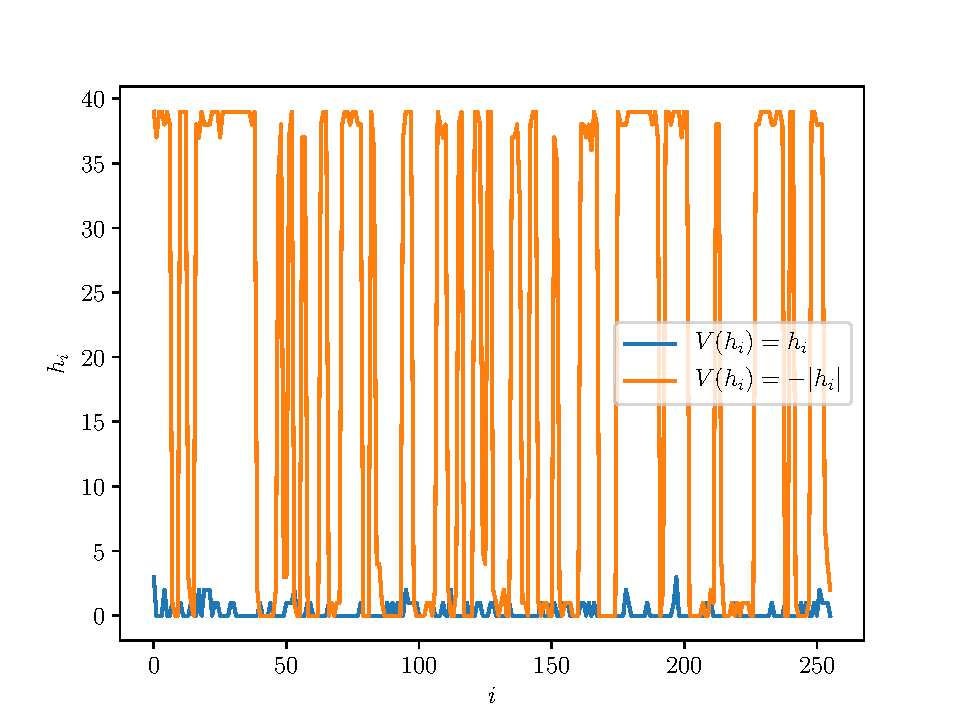
\includegraphics[width=\linewidth]{chap4/comp-potentiels-chimiques.pdf}
	\end{minipage}
	\begin{minipage}[t]{0.5\linewidth}
		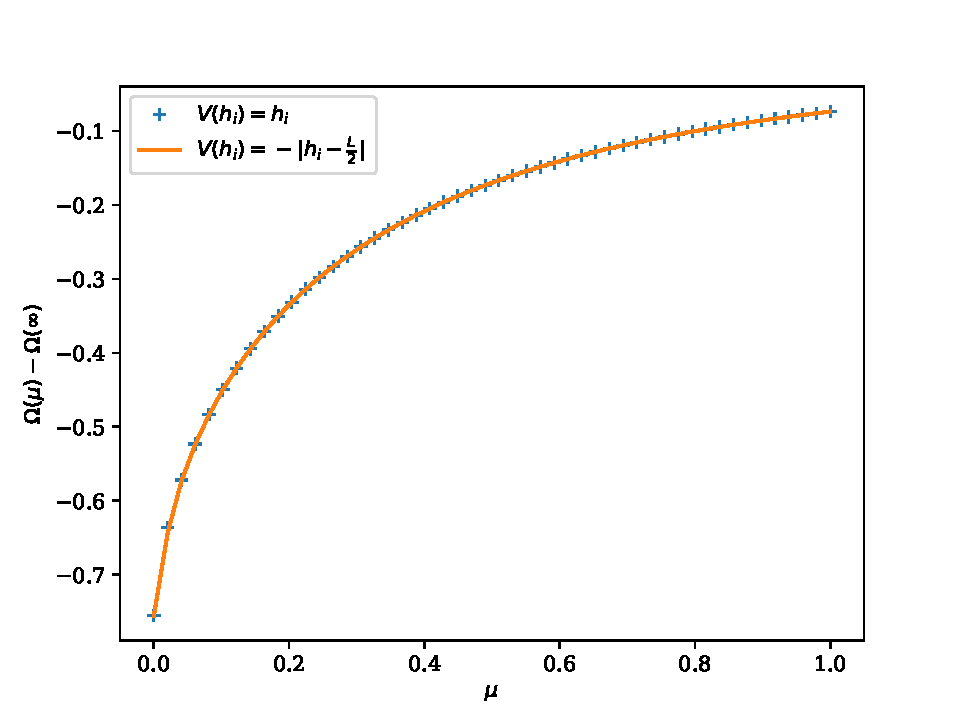
\includegraphics[width=\linewidth]{chap4/free-ene-potentiels.pdf}

	\end{minipage}
    \caption{Configuration possible du système à $\beta=1$ et $\mu$ élevé ($\mu=2$) pour les deux types de potentiel (gauche) ; énergie libre en fonction de $\mu$ à laquelle on a retiré l'énergie libre de la configuration limite pour les deux types de potentiel (droite).}
    \label{comp-potentiels-chimiques}
\end{figure}

Dnas la limite $\mu \rightarrow \infty$, on a donc un système éparpillé à $h=0$ et $h=L$. On a la matrice de transfert
\begin{align}
T= e^{-\beta \mu \frac{L}{2}}
  \begin{pmatrix}
    1 & e^{-\beta  J L} \\
    e^{-\beta  J L} & 1
  \end{pmatrix}
\end{align}
Les valeurs propres sont $\lambda_\pm = e^{- \beta \mu \frac{L}{2}}( 1 \pm e^{-\beta J L})$, ce qui nous donne dans la limite thermodynamique l'énergie libre 
\begin{align}
  \Omega(\mu \rightarrow \infty) = \mu \frac{L}{2}
\end{align}
Il est donc aisé de calculer l'énergie libre pour un champ donné grâce à l'intégration
\begin{align}
        \Omega(\beta,L,\mu) = -\Omega(\beta,L,\infty) + \int_{\mu}^\infty d\mu'  < \sum_i V(h_i) >_{\beta,L,\mu'} 
\end{align}
Cette méthode d'intégration est particulièrement adaptée aux modèles sur réseau où l'on connait la limite du système soumis à un potentiel extrême. Dans le cas du modèle SOS, il est possible de diagonaliser directement la matrice de transfert pour $\mu=0$, et ainsi obtenir
\begin{align}
        \Omega(\beta,L,\mu) =\Omega(\beta,L,0) + \int_{0}^\mu d\mu'  < \sum_i V(h_i) >_{\beta,L,\mu'} 
\end{align}
Pour petits champs, cette intégration est plus rapide.

Dans la figure \ref{comp-potentiels-chimiques} on remarque que la différence d'énergie libre $\Omega(\beta,\mu,L)$ et $\Omega(\beta,\infty,L)$ est la même dans nos deux systèmes. Cette équivalence entre les deux modèles nous autorise à mesurer la variation de l'énergie libre (et ainsi l'effet Casimir) via l'intégration de la quantité $<\sum_i V(h_i)>$ dans le cas où la dynamique conserve le paramètre d'ordre $<\sum_i h_i>$. 
Dansla figure \ref{casimir-kaw-glau} nous montrons les différences dans les effets de taille finie selon l'ensemble thermodynamique choisit. 

\begin{figure}
    \centering
	\includegraphics[width=0.5\linewidth]{example-image-b}
	\caption{Effet Casimir pour Kawasaki avec cisaillement pour différent $\mu$}
	\label{casimir-kaw-glau}
\end{figure}



%%%%%%%%%%%%%%%%%%%%%%%%%%%%%%%
    \section{Conclusion}
%%%%%%%%%%%%%%%%%%%%%%%%%%%%%%%	
	
Nous avons également vu une manière d'obtenir la fonction universelle de la force de Casimir critique via le découplage progressif d'une couche du système, afin que dans la limite où $L' \gg 1$, ce découplage s'apparent à la dérivée discrète de l'énergie libre (section \ref{sec-transition}). Dans le chapitre \ref{chap-sos}, nous étudions une manière moins générale d'obtenir cette énergie libre par de l'intégration d'une autre vari
